\newglossaryentry{CSV}
{
  name=CSV-Datei,
  description={\textit{Comma-separated values}\newline Hierbei werden Messungen in einer Textdatei durch Zeilenumbrüche und einzelne Werte durch Beistriche getrennt}
}

\newglossaryentry{CPU}
{
  name=CPU,
  description={\textit{Central Processing Unit}\newline
  	der Hauptprozessor}
}

\newglossaryentry{Ampere}
{
  name=Ampere,
  description={die SI-Basiseinheit der elektrischen Stromstärke}
}

\newglossaryentry{Hertz}
{
  name=Hertz,
  description={die SI-Basiseinheit für die Frequenz\newline Sie gibt die Wiederholungen pro Sekunden an (hier: Wechsel zwischen \emph{Strom} und \emph{kein Strom} in der \gls{CPU} pro Sekunde}
}

\newglossaryentry{Volt}
{
  name=Volt,
  description={die SI-Basiseinheit der elektrischen Spannung}
}

\newglossaryentry{gpio}
{
  name=GPIO,
  description={\emph{General Purpose Input/Output}\newline Kontakte auf der \gls{Platine}, die softwareseitig für verschiedene Zwecke angesteuert werden können\newline \zB: Auslesen von Sensoren, Ansteuern von Displays}
}

\newglossaryentry{Kernelmodul}
{
  name=Kernelmodul,
  description={ein Programm, welches in das Betriebssystem geladen werden kann und oft zur Kommunikation mit Hardware verwendet wird}
}

\newglossaryentry{1-Wire}
{
  name=1-Wire,
  description={ein \gls{Bus}-System zur einfachen Kommunikation mit Sensoren},
  sort=One-Wire
}

\newglossaryentry{Ohm}
{
  sort=Ohm,
  description={Das Ohm \emph{ist die abgeleitete SI-Einheit des elektrischen Widerstands}\footcite{wiki:ohm}},
  name={\ensuremath{\Omega}}
}

\newglossaryentry{Pascal}
{
  name=Pascal,
  description={ist die Einheit des (Luft-)Drucks}
}


\newglossaryentry{C}
{
  name=C,
  description={eine sehr weit verbreitete Programmiersprache\newline Hier wird sie oft zum Auslesen der Sensoren verwendet, da sie sehr schnell ausgeführt wird}
}

\newglossaryentry{Bus}
{
  name=Datenbus,
  description={\emph{System zur Datenübertragung zwischen mehreren Teilnehmern über einen gemeinsamen Übertragungsweg, bei dem die Teilnehmer nicht an der Datenübertragung zwischen anderen Teilnehmern beteiligt sind.}\footcite{wiki:bus}}
}
\newglossaryentry{I2C}
{
  name=I\textsuperscript{2}C,
  description={\textit{Inter-Integrated Circuit} (auf Deutsch gesprochen: \textit{I-Quadrat-C})\newline ein sehr weit verbreiteter \gls{Bus}}
}

\newacronym{voc}{VOC}{volatile organic compound (dt. Flüchtige organische Verbindungen)}

\newglossaryentry{Javascript}
{
  name=JavaScript,
  description={eine Skriptsprache für dynamische Inhalte in Webseiten}
}

\newglossaryentry{Flickr}
{
  name=Flickr,
  description={ist eine Online-Plattform, auf der Fotos hochgeladen und veröffentlicht werden können}
}

\newglossaryentry{Github}
{
  name=Github,
  description={\emph{ein webbasierter Hosting-Dienst für Software-Entwicklungsprojekte}\footcite{wiki:github}}
}

\newglossaryentry{Python}
{
  name=Python,
  description={ist eine 1991 entwickelte Programmiersprache, deren Fokus auf Programmlesbarkeit liegt.\footcite{python}$^,$\footcite{python_manual}{}}
}

\newglossaryentry{Bash}
{
  name=Bash,
  description={\textit{Bourne-again shell}\newline ist die heute unter Linux am häufigsten verwendete \gls{Shell}}
}

\newglossaryentry{Shell}
{
  name=Shell,
  description={ist eine Schnittstelle, über die der Benutzer Kommandos an den Computer schicken kann}
}

\newglossaryentry{Einplatinencomputer}
{
  name=Einplatinencomputer,
  description={ein vollständiges Computersystem, welches auf einer einzelnen \gls{Platine} zusammengefasst ist}
}

\newglossaryentry{LC-Display}
{
  name=LC-Display,
  description={\emph{liquid crystal display}\newline Flüssigkristallbildschirm}
}

\newglossaryentry{Platine}
{
  name=Platine,
  description={auch genannt Leiterplatte\newline
  ein Träger für elektrische Bauteile\newline
  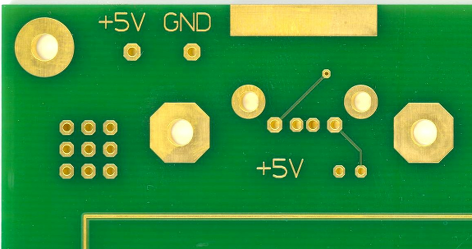
\includegraphics[width=4cm]{figures/platine.png}\footcite{platine}
    	}
}

\newglossaryentry{Streifenplatine}
{
  name=Streifenplatine,
  plural=Streifenplatinen,
  description={eine \gls{Platine}, bei der die Kontakte streifenförmig miteinander verbunden sind.\newline
  
\includegraphics[width=4cm]{figures/streifenplatine.png}\footcite{streifenplatine}
  	}
}

\newglossaryentry{LED}
{
  name=LED,
  description={\emph{light-emitting diode}\newline Licht abgebende Diode}
}

\newglossaryentry{Geraetedatei}
{
  name=Gerätedatei,
  description={eines der grundlegenden Prinzipien von diversen Linux-Betriebssystemen ist \emph{Everything is a file}.\newline
  Daher können auf Festplatten, Schnittstellen und Informationen über das System einfach über das Auslesen von Dateien zugegriffen werden.
  }
}

\newglossaryentry{Standardabweichung}
{
  name=Standardabweichung,
  description={ein Maß für die Streuung von Werten}
}

\newglossaryentry{Steckbrett}
{
  name=Steckbrett,
  description={hierauf können schnell Schaltungen aufgebaut und getestet werden}
}

\newglossaryentry{Linux-Distribution}
{
  name=Linux-Distribution,
  plural=Linux-Distributionen,
  description={Es gibt nicht nur ein \emph{Linux}, sondern eine sehr große Menge\footnote{siehe diese Grafik: \href{http://de.wikipedia.org/wiki/Datei:Linux_Distribution_Timeline.svg}{de.wikipedia.org/wiki/Datei:Linux\_Distribution\_Timeline.svg}} Betriebssysteme, welche alle auf dem ursprünglichen \emph{Linux}-Kernel basieren.}
}

\newglossaryentry{Gnuplot}
{
  name=Gnuplot,
  description={ein Programm \emph{zur grafischen Darstellung von Messdaten und mathematischen Funktionen}\footcite{wiki:gnuplot}}
}